Im Menü Data-Inputs gibt es den Punkt Supplierungen anlegen, hier können, wie der Name schon sagt, neue Supplierungen angelegt werden. (siehe \autoref{fig:instr_substitudes_dataInput}) Klickt man auf diesen Punkt so erscheint die Eingabemaske.(siehe \autoref{fig:instr_substitudes_subNoFree}) Für den Super-User erscheint zuerst eine Auswahl zwischen den einzelnen Abteilungen. (siehe \autoref{fig:instr_substitudes_subSuUs}) Erst nach der Auswahl der Abteilungen kommt ein Super User zur Eingabemaske.\\
\begin{figure}[H]
\centering
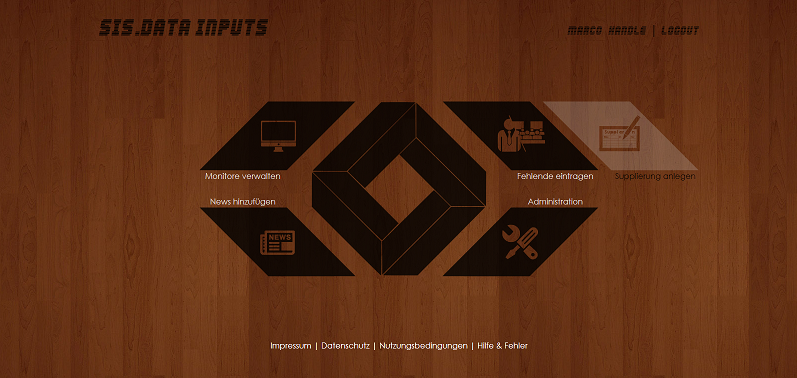
\includegraphics[keepaspectratio=true, width=17cm]{images/screenshots/data-inputs_substitudes.png}
\caption{Data-Input-Menü}
\label{fig:instr_substitudes_dataInput}
\end{figure}
\begin{figure}[H]
\centering
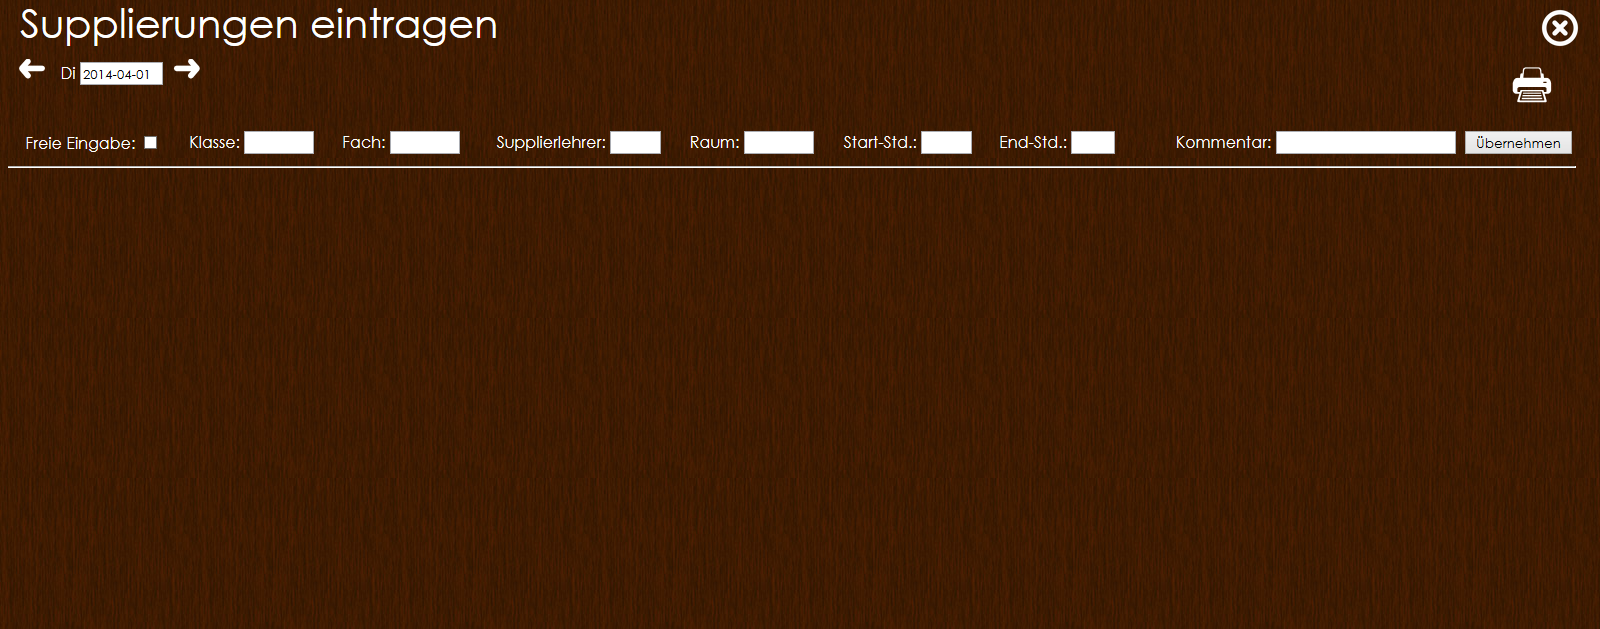
\includegraphics[keepaspectratio=true, width=17cm]{images/screenshots/substitudes_nofree.png}
\caption{Eingabemaske normal}
\label{fig:instr_substitudes_subNoFree}
\end{figure}
\begin{figure}[H]
\centering
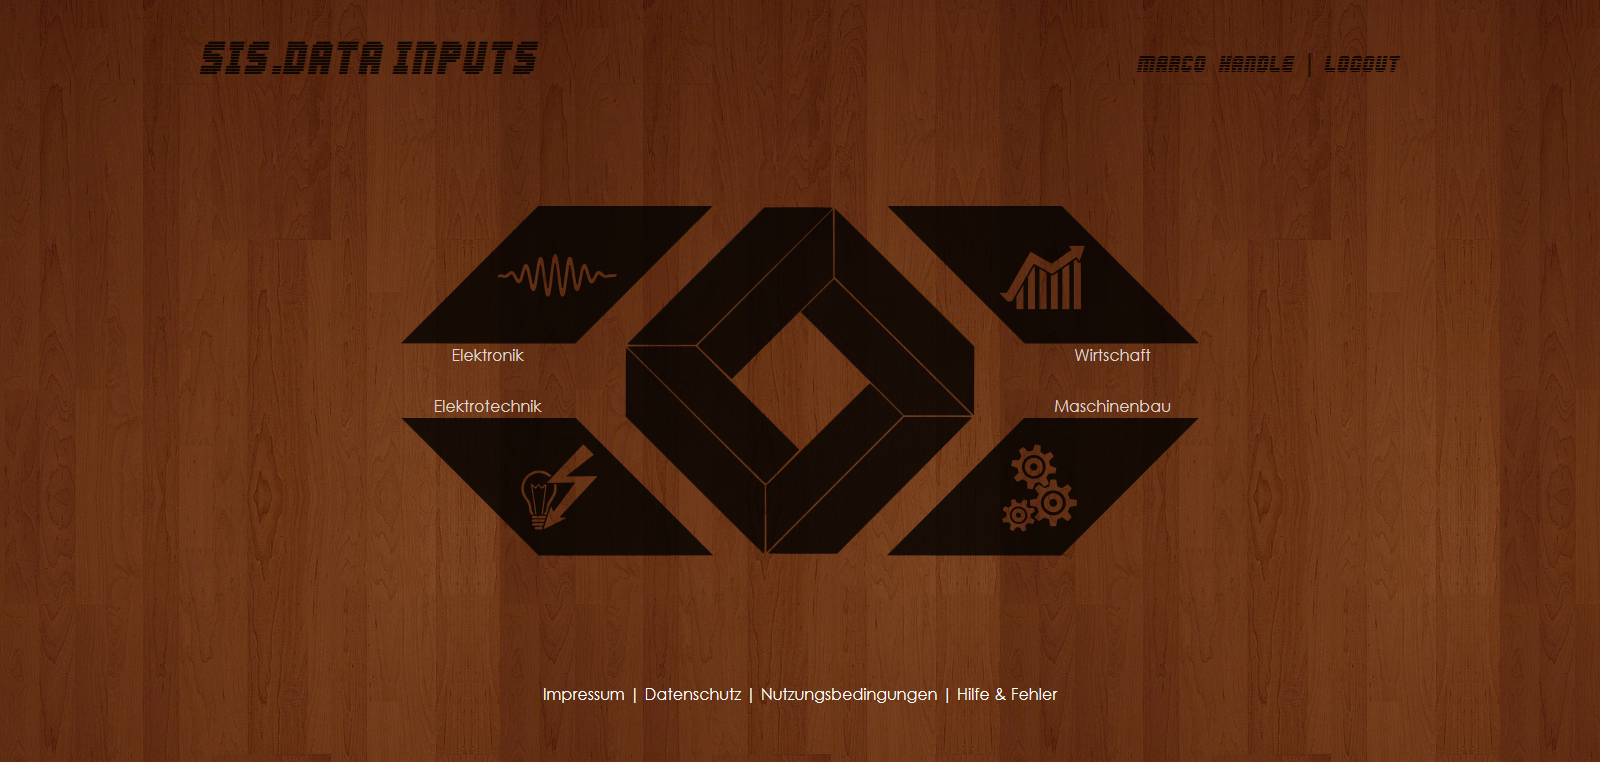
\includegraphics[keepaspectratio=true, width=17cm]{images/screenshots/substitudes_sections.png}
\caption{Super User Auswahl}
\label{fig:instr_substitudes_subSuUs}
\end{figure}
Die Datumsauswahl funktioniert exakt auf die selbe Weise wie bei den fehlenden Lehrern/Schülern. Bei Unklarheiten siehe \autoref{sec:instr_admin_absentees}.\\
Insgesamt gibt es 4 Grundlegende Eintragungsvarianten:
\begin{itemize}
	\item Normale Eingabe\\
		siehe \autoref{sec:instr_admin_sub_noFree}
	\item Freie Eingabe\\
		siehe \autoref{sec:instr_admin_sub_Free}
		\begin{itemize}
			\item Stunde verschieben\\
				siehe \autoref{sec:instr_admin_sub_move}
			\item Stunde hinzufügen\\
				siehe \autoref{sec:instr_admin_sub_add}
			\item Stunde entfällt\\
				siehe \autoref{sec:instr_admin_sub_remove}
		\end{itemize}
\end{itemize}
\subsection{Normale Eingabe}\label{sec:instr_admin_sub_noFree}
Diese Eingabe, kann dann gut verwendet werden, wenn in einer Klasse ein Lehrer fehlt, dieser muss jedoch als fehlend zuvor eingetragen werden. Fehlen mehrere Lehrer in der selben Klasse zur selben Zeit, dann wird diese Eingabe problematisch. Dann muss auf eine andere Eingabeform zurückgegriffen werden.\\
Prinzipiell funktioniert diese Eingabevariante nur wenn der Lehrer in dieser Stunde fehlt und dann eine Supplierung eingetragen werden soll. Mit dieser Eingabevariante kann jedoch nur eine Supplierung eingetragen werden, es ist nicht möglich die Stunde zu verschieben oder ausfallen zu lassen.\\\\
Von den Eingabefeldern ist die Eingabe der Klasse und des Supplierlehrers verpflichtend. Weiteres muss die Start- und End-Stunde angegeben werden. Fach, Raum und Kommentar sind optionale Eingabefelder. (siehe \autoref{fig:instr_substitudes_subNoFree})
\subsection{Freie Eingabe}\label{sec:instr_admin_sub_Free}
Diese Eingabe ist dafür da, dass man auch eine Supplierung eintragen kann wenn der ursprüngliche Lehrer nicht fehlt. Diese Eingaben funktionieren immer. Um diese Methode zu wählen muss ein Hacken bei freie Eingabe setzen. Anschließend kommen neue Felder hinzu. Direkt unter der Check Box gibt es drei Radio Buttons. Diese werden zur Auswahl der Eingabemethode bei der Freien Eingabe verwendet. Wird ein Radio Button ausgewählt ändert sich die Konstellation der Eingabefelder.
\subsubsection{Verschieben}\label{sec:instr_admin_sub_move}
In dieser Eingabevariante können Stunden einer Klasse innerhalb eines Tages verschoben werden. Außerdem muss diese Variante auch verwendet werden, wenn zum Beispiel 2 oder mehr Lehrer in einer Klasse zur selben Zeit fehlen und genau geregelt ist, welcher Supplierlehrer welchen Lehrer vertritt. Da es jedoch keine Verschiebung ist, sondern eigentlich nur eine Vertretung, muss in diesem Fall die Start- und Endstunde und die Ursprüngliche Start- und End-Stunde gleich sein. Damit die Stunde wieder zur selben Zeit stattfindet. Sie kann auch dazu verwendet werden um eine vorhandene Stunde zu kürzen. Dann muss die ursprüngliche Stunde angegeben werden und kann dann mit der neuen Start- und End-Stunde hinzugefügt werden. So kann eine Stunde, die von der 1-4 dauert, in eine Stunde die von der 2-3 dauert, verkürzt werden.\\
Die Form der Eingabemaske entspricht im wesentlichen, der Form der normalen Eingabe, jedoch sind 3 Felder hinzugekommen. (siehe \autoref{fig:instr_substitudes_subMove}) Diese dienen dazu die ursprüngliche Stunde festzulegen. Wird eine Verschiebung eingetragen wird diese von der ursprünglichen Position entfernt.\\
Pflichtfelder sind die Klasse, Start- und End-Stunde, ursprüngliche Start- und End-Stunde und ursprüngliche Lehrer. Die restlichen Felder sind optional. Wird eines dieser optionalen Felder nicht eingetragen, dann werden die Daten der ursprünglichen Stunde verwendet. Sobald Verschiebung ausgewählt wurde, wird automatisch in das Kommentarfeld "Verschiebung von" eingetragen.
\begin{figure}[H]
\centering
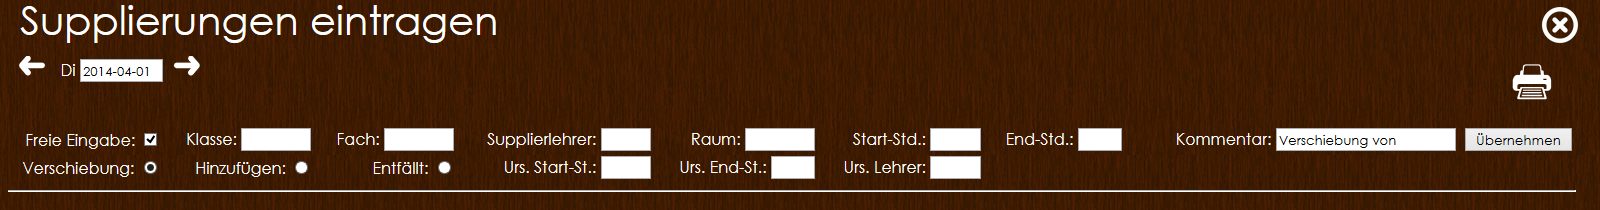
\includegraphics[keepaspectratio=true, width=17cm]{images/screenshots/substitudes_move.png}
\caption{Eingabemaske Verschiebung}
\label{fig:instr_substitudes_subMove}
\end{figure}
\subsubsection{Hinzufügen}\label{sec:instr_admin_sub_add}
Diese Variante kann dazu verwendet werden, falls zum Beispiel eine Stunde von einem anderen Tag auf diesen Tag verschoben wird. Diese Variante kann auch einfach dazu verwendet werden irgendwo eine Stunde einzufügen. Wenn diese Eingabevariante gewählt wird, überschreibt der neue Eintrag den ursprünglichen Stundenplan der Klasse.\\
Die Eingabemaske ist identisch mit, der der normalen Eingabe. (siehe \autoref{fig:instr_substitudes_subAdd} Pflichtfelder sind in dieser Variante Klasse,Fach,Supplierlehrer (in diesem Fall der Lehrer)und die Start- und End-Stunde. Raum und Kommentar sind optionale Felder.
\begin{figure}[H]
\centering
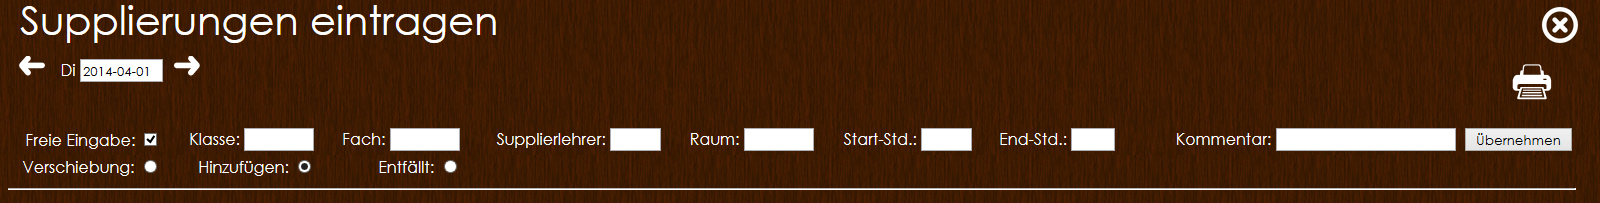
\includegraphics[keepaspectratio=true, width=17cm]{images/screenshots/substitudes_add.png}
\caption{Eingabemaske Hinzufügen}
\label{fig:instr_substitudes_subAdd}
\end{figure}
\subsubsection{Entfallen}\label{sec:instr_admin_sub_remove}
Diese Variante wird dazu benötigt eine vorhandene Stunde ausfallen zu lassen. Dabei wird die Stunde im Stundenplan der Schüler bzw. Lehrer nicht mehr angezeigt. Wird Entfällt ausgewählt, dann wird in das Kommentarfeld automatisch Entfällt eingefügt.\\
Die Eingabemaske ist auf das nötigste reduziert. (siehe \autoref{fig:instr_substitudes_subRemove}) Die Pflichtfelder sind Klasse, ursprüngliche Start- und End-Stunde und der ursprüngliche Lehrer. Das Kommentarfeld ist optional.
\begin{figure}[H]
\centering
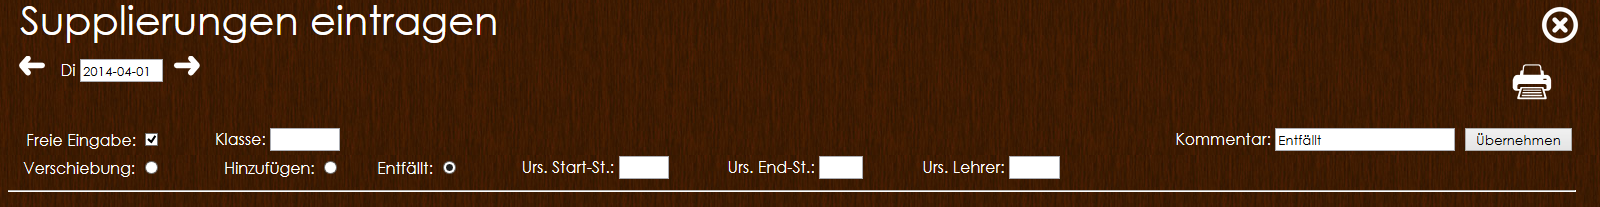
\includegraphics[keepaspectratio=true, width=17cm]{images/screenshots/substitudes_remove.png}
\caption{Eingabemaske Entfallen}
\label{fig:instr_substitudes_subRemove}
\end{figure}
\subsection{Fehler}
Wenn in die Textboxen Werte eingegeben werden, welche nicht in unserer Datenbank vorhanden sind, dann wird ein Fehler zurückgegeben. Dazu erscheint ein Pop-Up indem der Name der Fehlerhaften Textbox geschrieben ist. Dieses Pop-Up muss mit OK bestätigt werden, anschließend muss die Eingabe erneut erfolgen.\\
Ein weiterer Fehler kann sein, dass bei der normalen Eingabe eine Supplierung angelegt werden will, ohne dass der ursprüngliche Lehrer fehlt. Dabei wird ein Fehler zurückgegeben und der Trennstrich unter der Supplierung wird rot. Die zuvor eingegebenen Werte werden in die Textbox eingefügt. Dies kann auch bei einer freien Eingabe auftreten, zum Beispiel wenn die ursprüngliche Stunde nicht gefunden wird, dann wird auch dieser Fehler ausgegeben. (siehe \autoref{fig:instr_substitudes_fail})
\begin{figure}[H]
\centering
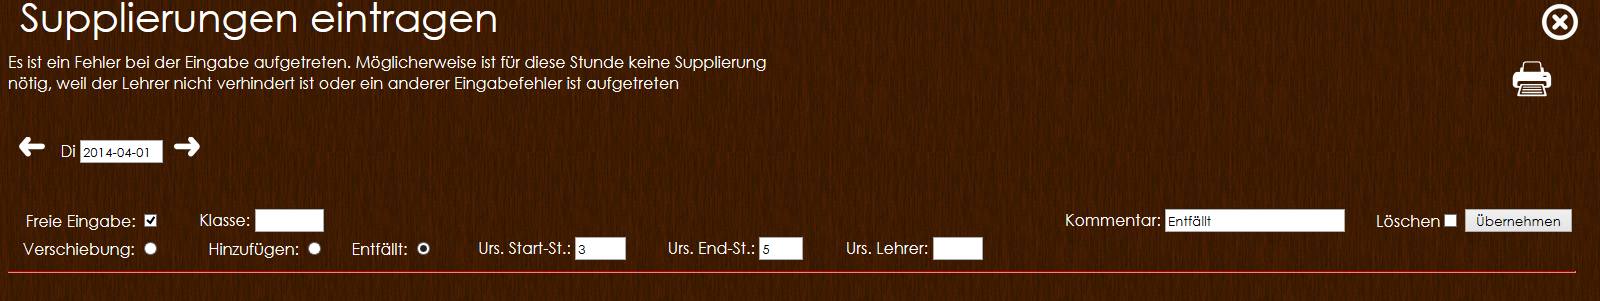
\includegraphics[keepaspectratio=true, width=17cm]{images/screenshots/substitudes_fail.png}
\caption{Eingabemaske Entfallen}
\label{fig:instr_substitudes_fail}
\end{figure}
\subsection{Verändern}
Soll eine vorhandene Supplierung verändert werden, so kann das auf einfache weise gemacht werden. Dabei kann einfach der Eintrag verändert werden. Ist alles nach den neuen Wünschen angepasst, so muss auf Übernehmen geklickt werden um die Supplierung zu übernehmen.
\subsection{Löschen}
Soll eine Supplierung gelöscht werden, so muss der HAcken bei Löschen bei der gewünschten Supplierung gesetzt werden und anschließend muss auf Übernehmen geklickt werden. Anschließend wird die Supplierung unwiderruflich gelöscht.